\documentclass{beamer}
\usepackage{physics}
\usepackage{amsmath}
\usepackage{tikz}
\usepackage{mathdots}
\usepackage{yhmath}
\usepackage{cancel}
\usepackage{color}
\usepackage{siunitx}
\usepackage{array}
\usepackage{multirow}
\usepackage{amssymb}
\usepackage{textcomp, gensymb}
\usepackage{tabularx}
\usepackage{extarrows}
\usepackage{booktabs}
\usetikzlibrary{fadings}
\usetikzlibrary{patterns}
\usetikzlibrary{shadows.blur}
\usetikzlibrary{shapes}
\usepackage[style=verbose,backend=bibtex]{biblatex}
\addbibresource{arpes.bib}
\addbibresource{green.bib}
\usepackage{listings}
\usepackage{hyperref}

\newcommand{\pair}[1]{\langle #1 \rangle}
\DeclareMathOperator{\ee}{e}
\DeclareMathOperator{\ii}{i}

\newcommand{\concept}[1]{\textbf{#1}}
\newcommand{\corpus}[1]{\emph{#1}}

%Information to be included in the title page:
\title{Do Americans really speak ``English''?}
\author{Jinyuan Wu}

\usetheme{Madrid}

\begin{document}
    
\frame{\titlepage}

\begin{frame}
\frametitle{Variation of English}

\begin{columns}
    
\begin{column}{0.5\textwidth}
    Besides English as we know it, 
    what do Americans speak?

    \begin{itemize}
        \item Spanish? 
        \item English\emph{es}!
    \end{itemize}
\end{column}

\begin{column}{0.43\textwidth}
    \begin{center}
        
\includegraphics[width=\textwidth]{pics/i-dont-know-nothing-i-think-and-glad-of-it-quote-1.jpg}
    \end{center}
\end{column}

\end{columns}

\footnotetext{
        Picture from \href{http://www.picturequotes.com/i-dont-know-nothing-i-think-and-glad-of-it-quote-14372}{Picture Quotes}.
}

\end{frame}

\begin{frame}
\frametitle{Variation of English}

Yale is famous for its humanities,
and thanks for a bunch of people in this building,
we have \dots

\begin{center}
    
\includegraphics[width=0.7\textwidth]{pics/yale-grammar-variation-logl.PNG}
\end{center}

\begin{center}
    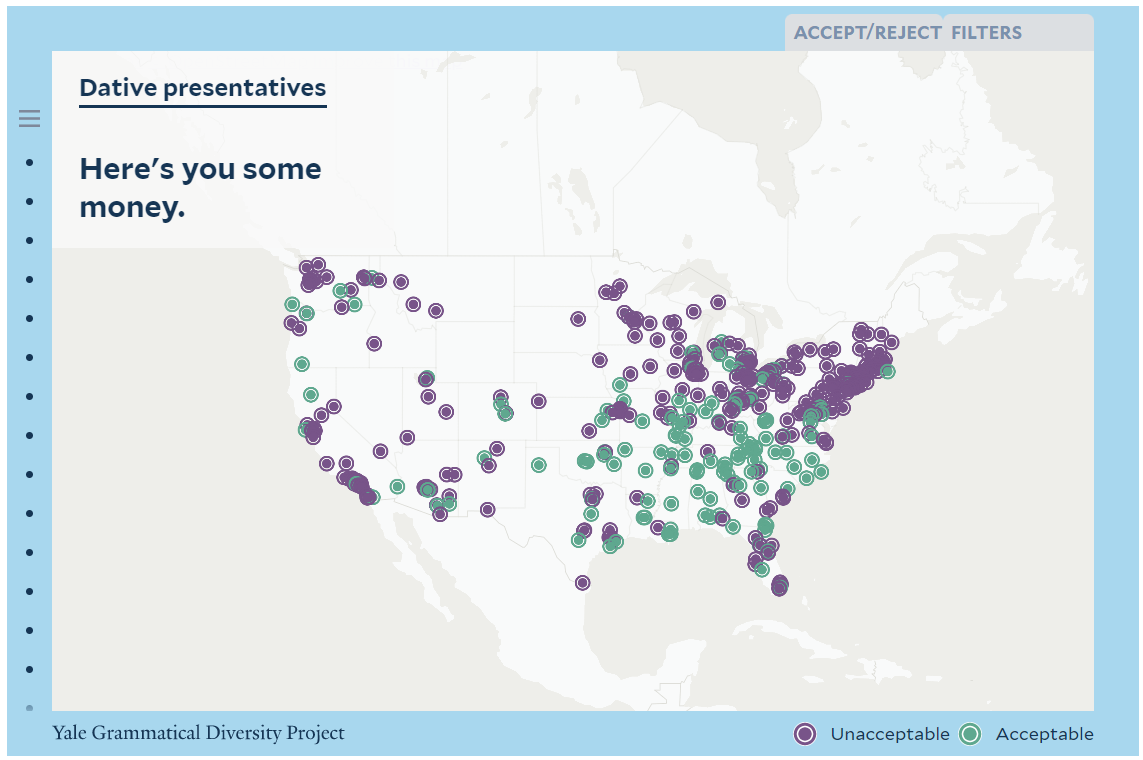
\includegraphics[width=0.6\textwidth]{pics/yale-grammar-map-1.PNG}
\end{center}

\end{frame}

\begin{frame}
\frametitle{Example: \corpus{Here's you a piece of pizza}}

On the page about \href{https://ygdp.yale.edu/phenomena/dative-presentatives}{dative presentatives}:

\textbf{Who says it}

\begin{center}
    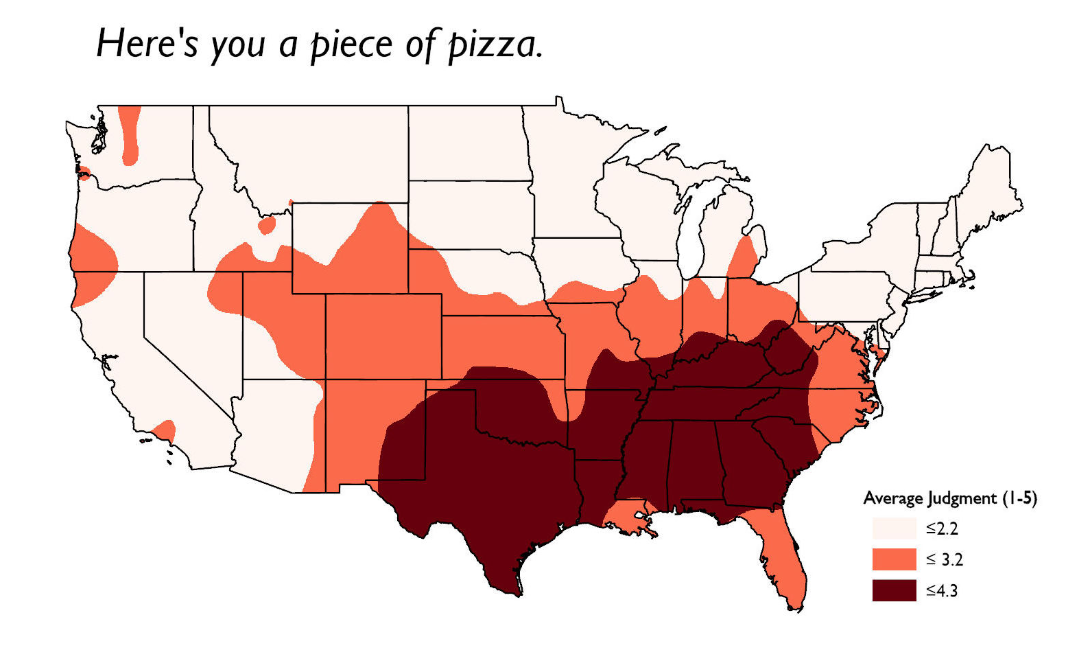
\includegraphics[width=0.5\textwidth]{maps/here-is-you-a-piece-of-pizza.PNG}
\end{center}    

\textbf{Syntactic environments}

\begin{itemize}
    \item {[\corpus{Here's} [\corpus{John/you}]$_{\text{dative:NP}}$ \corpus{a glass of iced-tea}]$_{\text{existential, declarative}}$} 
    \item {[\corpus{Where's} [\corpus{me}]$_{\text{dative}}$ \corpus{a screwdriver}]$_{\text{existential, interrogative}}$}
\end{itemize}

\end{frame}

\begin{frame}
\frametitle{Example: negative concord}

On the page about \href{https://ygdp.yale.edu/phenomena/negative-concord}{negative concord}:

\textbf{Who says this}

\begin{center}
    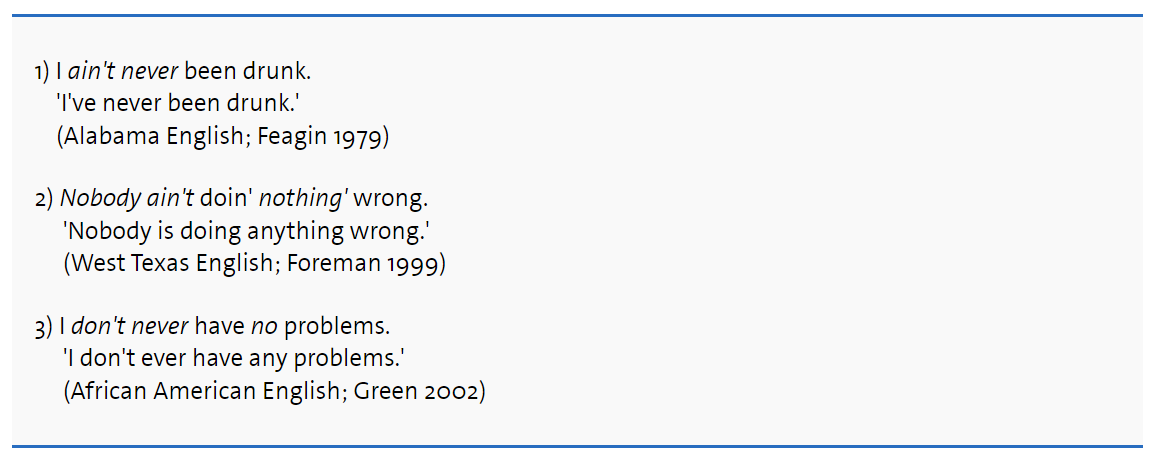
\includegraphics[width=0.8\textwidth]{pics/content-example-2.PNG}
\end{center}    

\textbf{Types of negative concord}

\begin{itemize}
    \item Negative adverb after negated auxiliary: \corpus{I ain't never lost a fight}
    \item Negative pronoun with negated auxiliary: \corpus{Nobody couldn't handle him}
    \item Even in complement clause: \corpus{I don't feel like [nobody pets me]}
\end{itemize}

\end{frame}

\begin{frame}
\frametitle{Why recording these}

\begin{itemize}
    \item General linguistics:
    \begin{itemize}
        \item Providing evidences for universal constraints on \emph{possible} natural languages
        \item Providing evidences for typological \emph{tendencies} (not absolute) 
    \end{itemize}
    \item English philology:
    \begin{itemize}
        \item Simply for fun: stamp collecting is also interesting!
        \item More expressive language
    \end{itemize}
\end{itemize}    

\end{frame}

\begin{frame}
\frametitle{Conclusion}

\begin{itemize}
    \item English dialects have exotic constructions
    \item They can be found in \url{https://ygdp.yale.edu/}!
\end{itemize}    

\end{frame}

\end{document}